\chapter{Rapport d'activité}

\section{Organisation du travail}
        
\subsection{Communication}

        La communication s'est au départ faite au travers de réunions hebdomadaires au cours desquelles le cahier des charges a été défini auprès de M. Meynard.
        
        Une fois le cahier des charges défini et rendu, le but suivant a été de déterminer quel langage et quel bibliothèque d'affichage graphique sélectionner pour le projet et ainsi être conscient des avantages et des limites des éléments choisis.
        
        Ensuite, l'objectif suivant a été de définir une maquette du logiciel afin de savoir quelles seront les fonctionnalités retenues, la manière de les exploiter et quel organisation visuelle du logiciel sera retenue. C'est ainsi qu'a été définie la maquette qui comporte une interface simple avec une barre d'outils, une vue principale sur le côté droit avec le système d'éditeur de texte, une vue secondaire sur la gauche avec la vue arborescente du modèle XML du fichier présenté par l'utilisateur et enfin la fenêtre de log associé au différents messages liés à l'utilisation de l'éditeur, par exemple, des erreurs de schéma.
        
        Il fallait enfin définir l'organisation du travail au sein du groupe avec des tâches définies et mettre un place un plan de travail, c'est donc Stéphane WOUTERS, le chef du projet, qui a mis en place le gestionnaire de projet, a décidé des moyens de communication et qui a défini le premier objectif de développement : l'apprentissage de la librairie.
        
        Puis la phase d'apprentissage et de développement commença, il fallait alors découvrir et apprendre le framework utilisé, et commencer à développer pour le projet, la communication s'est donc faite au travers de messages sur Google Hangouts, de mails, de commentaires via le gestionnaire de projet et de communication orale dans une salle informatique de la faculté.
        
        \subsection{Répartition des tâches}

\section{Outils de développement}

\subsection{Langage et bibliothèques}

Nous avons décider d'utiliser C++ comme langage pour ce projet, nous avions également l'option d'utiliser Java, mais C++ étant un nouveau langage pour nous, il a été retenu pour parfaire nos connaissances. Il a ensuite été décidé d'utiliser Qt comme bibliothèque d'interface graphique. Nous avions à nouveau un choix à faire, mais Qt a été préféré par rapport à GTK, l'autre grande bibliothèque d'affichage de fenêtres, il est en effet plus documenté et utilisé, et n'embarque pas uniquement des utilitaires d'affichages, mais également un grand nombre d'outils et classes qui nous faciliterons grandement la tâche.
\paragraph{}
Qt a également l'avantage d'être multi-plateforme, le code produit est en théorie compilable sur les systèmes d'opération majeurs. C'est alors le gestionnaire de fenêtre de la plateforme cible qui sera utilisé comme on peut le voir figures \ref{apparence_linux}, \ref{apparence_mac} et \ref{apparence_windows}, on a donc des applications qui se fondent dans l'environnement natif et respectent l'esthétique du système sans travail supplémentaire de la part du développeur.

\begin{figure}[h!]

\begin{minipage}[b]{\linewidth}
\centering 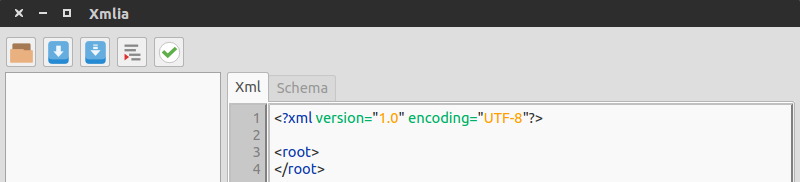
\includegraphics[scale=0.5]{images/apparence_linux.png}
\caption{Apparence sous Linux}
\label{apparence_linux}
\end{minipage}
\begin{minipage}[b]{\linewidth}   
\centering 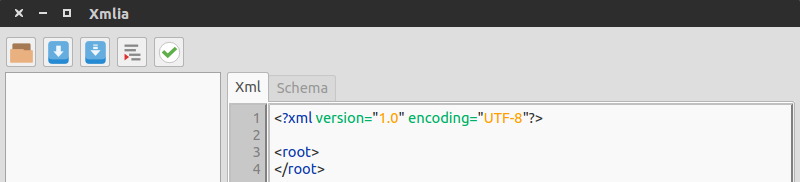
\includegraphics[scale=0.5]{images/apparence_linux.png}
\caption{Apparence sous Mac Os}
\label{apparence_mac}
\end{minipage}
\begin{minipage}[b]{\linewidth}
\centering 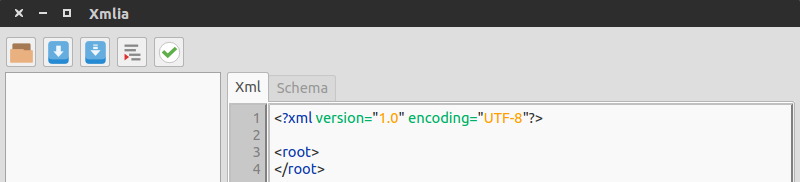
\includegraphics[scale=0.5]{images/apparence_linux.png}
\caption{Apparence sous Windows}
\label{apparence_windows}
\end{minipage}
\end{figure}

\paragraph{}

Qt DANS SA GRANDEUR EMBARQUE PLEIN DE MODULES LOUÉ SOIT Qt !

\subsection{IDE}
Nous avons naturellement utilisé Qt Creator comme IDE, c'est en effet l'IDE fourni avec Qt, il intègre donc nativement toutes les opérations spécifiques à la création et la compilation d'un projet sous Qt. Il intègre également toutes les fonctionnalités que l'on pourrait attendre d'un IDE digne de ce nom.
\paragraph{}
Qt propose en plus un éditeur d'interface graphique nommé Qt Designer qui permet de créer des interfaces très simplement avec du glisser-déposer notamment et d'ensuite les intégrer dans une application Qt. Nous avons cependant fait le choix de ne pas l'utiliser, notre interface est en effet suffisamment simple pour ne pas avoir recours à un outil supplémentaire.

\subsection{Gestionnaire de projet}
Le gestionnaire de projet utilisé est Bitbucket, un site Internet d'hébergement mutualisé supportant des projets utilisant Mercurial ou Git comme gestionnaire de versions. Dans le cas de Xmlia, Git a été retenu et utilisé.
\paragraph{}
Git a ici permis de gérer les accès et les mises à jour différents fichiers du projet, qu'ils soient du code ou du texte brut, comme par exemple pour le rapport du projet. Son utilité aura donc été de permettre une gestion des fichiers de manière formelle, avec des gestions de conflits de versions de fichier, par exemple avec un système de gestion de fichiers basique comme un FTP, si deux développeurs travaillent en accès concurrentiel sur le même fichier, chacun aura alors sa version du fichier et au moment de renvoyer le travail effectué sur le serveur FTP, un conflit de version surviendra, c'est pour cela que Git est utile en mettant en place des barrières empêchant ce genre de problèmes et proposant des solutions pour, par exemple, réunir les deux fichiers et qu'un développeur s'occupe de "merge" ces deux fichiers en un seul qui aura alors le code des deux développeurs. Un dernier point important à aborder est le fait qu'un envoi de code sur le serveur peut être annulé si par exemple une erreur d'utilisation de Git a été faite et que des fichiers auraient alors été modifiés rendant le projet non fonctionnel.
\paragraph{}       
Bitbucket est un service accessible depuis une page Web permettant la gestion de projet Git. Le service propose donc un serveur Git fonctionnel avec une interface Web très performante. Cette interface permet de gérer tous les projets auxquels on est rattaché, créer de nouveaux projets et gérer les droits liés à ces projets. Un nouveau projet a donc été créé sur le site au travers de l'interface puis les droits de modification du projet ont été données aux autres membres du groupe projet qui ont alors pu commencer à utiliser le Git du projet. Ajouté à cela, Bitbucket liste l'intégralité des différentes opérations effectuées sur le Git permettant un regard global et rapide sur toutes les réalisations et offre aux différents membres du groupe la possibilité d'écrire des commentaires sur chaque opération, les membres seront donc notifiés par e-mail de ce changement, ce qui aura été un moyen de communication très présent au cours de la phase de développement. De plus, une fonctionnalité très importante de Bitbucket pour la gestion de projets est le système de tickets qui est intégré à l'interface Web où chaque membre peut ajouter soit une tâche à effectuer ou un bug à corriger et l'affecter à un autre membre, cela permet alors d'avoir une communication plus claire et concise, donnant un regard des autres membres sur les tâches effectuées par le groupe, aussi en leur donnant la possibilité de commenter ces tickets et d'ajouter des informations nécessaires à la réalisation de la tâche, donnant alors un point de vue global sur l'avancement du projet.
\paragraph{}
La figure \ref{ticket_Bitbucket} montre par exemple un ticket concernant une fonction à coder avec une description précise et des commentaires afin de mettre l'accent sur le sens de la tâche à réaliser, afin d'avoir une compréhension plus claire du problème.
       
\begin{figure}[!h]
      \centering
      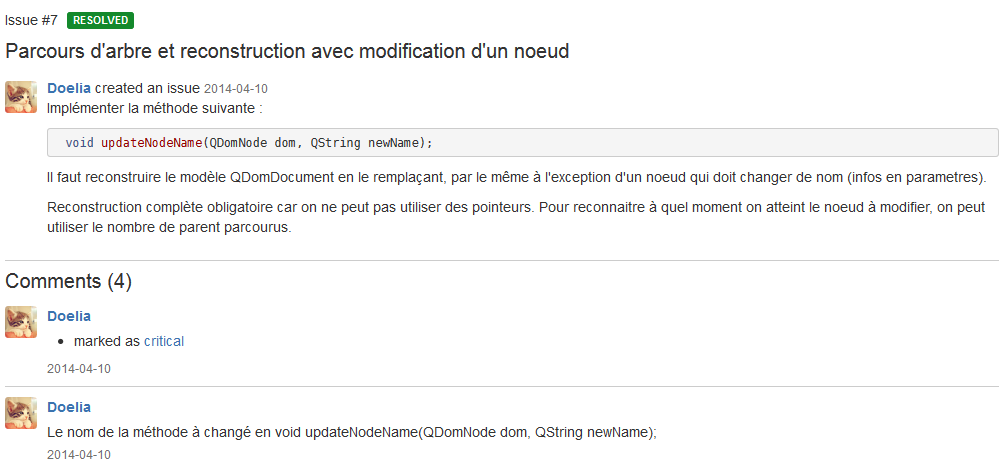
\includegraphics[scale=0.5]{images/bitbucket-exemple-issue.png}
      \caption[Exemple de ticket sur Bitbucket]{Exemple de ticket sur Bitbucket.}
      \label{ticket_Bitbucket}
\end{figure}

